% Preamble
\documentclass[a4paper,12pt]{article}

\usepackage[osf]{mathpazo} % palatino
\usepackage{ms}            % load the template
%\usepackage[round]{natbib} % author-year citations
\usepackage[superscript,biblabel]{cite} % for superscript citations
\usepackage{graphicx}
\usepackage{parskip} 
\usepackage{caption}
\usepackage{subcaption}
\usepackage{textcomp} % for parts per mille symbol     
\pagenumbering{arabic}    
\linespread{1.66}


% -------------------------------------------------------------------------------------------------------
% some custom commands

% Add support for highlighting
\usepackage{color}
\newcommand{\hilight}[1]{\colorbox{yellow}{#1}}

% -------------------------------------------------------------------------------------------------------

% Title page information
\title{Reconstructing the last known movements of one of Nature's giants}
% 90 characters max

\author{
  Clive N. Trueman$^{1}$, Andrew L. Jackson$^{2}$, Katharyn S. Chadwick$^{1}$,\\ Ellen J. Coombs$^{3,4}$,
  Richard C. Sabin$^{3}$ and Natalie Cooper$^{3*}$
}
\date{}
\affiliation{\noindent{\footnotesize
  $^1$ Ocean and Earth Science, University of Southampton Waterfront Campus, Southampton, SO14 3ZH, UK.\\
  $^2$ School of Natural Sciences, Trinity College Dublin, Dublin 2, Ireland.\\
  $^3$ Department of Life Sciences, Natural History Museum London, Cromwell Road, London, SW7 5BD, UK.\\ 
  $^4$ University College London, Gower Street, London, WC1E 6BT, UK.\\
}}

\vfill

%\runninghead{}
%\keywords{}
%}

% End of preamble

\begin{document}
\modulolinenumbers[1]   % Line numbering on every line

\mstitlepage

\parindent = 1.5em
\addtolength{\parskip}{.9em}
% Abstract 200 -300 words max
% \section{Abstract}
% general topic intro - 1 sentence
% intro to field - 2 sentences
% what we find/show - 1 sentence
% implications - 2-3 sentences. Results in context, how has the paper moved the field forward

\raggedright
% Need to edit
\paragraph{Understanding animal movements is crucial for effective conservation, especially as species ranges shift due to climate change\cite{runge2014conserving,robinson2009travelling}. 
Animal tissues housed in museum collections provide biochemical records of behaviour that can be used to reconstruct individual-level movements over long timescales and under historical climatic and ecological conditions\cite{newsome2010using}. 
Here we combine stable isotope analyses of baleen with novel agent-based simulation models, to reconstruct the movements of an iconic blue whale (\textit{Balaenoptera musculus}) that stranded off Ireland in 1891 and is now on display at the Natural History Museum, London. 
We identify two distinct phases in the whale's behaviour: repeated annual north-south migrations in sub-Arctic waters, and residency in subtropical waters. 
Subtropical residency is associated with isotopic signatures consistent with pregnancy and lactation in the year before the whale's death. 
These results supply the first quantitative multi-year records of historical migrations in individual blue whales, and suggest that blue whale residency and movement patterns in the North Atlantic have remained similar for hundreds of years, despite changing human pressures in the region. 
Historic tissue collections can provide unique insight into individual-level movement behaviours associated with changing climate, ecological conditions and anthropogenic pressures, and reveal aspects of life history. 
Combining biochemical tracers with simulation modeling unlocks the information recorded in these irreplaceable archives.}

%\section{Main text}
% 1500 words max (excludes refs title, authors, abstract, acknowledgements)
\newpage

Migratory species pose a particular challenge for conservation practitioners, because their effective conservation relies on protection at many, often distant, sites\cite{runge2014conserving}. 
Such species are also likely to be particularly vulnerable to climate change, as changes may impact various parts of their life cycle\cite{robinson2009travelling}. 
Dealing with these issues is difficult due to the relative scarcity of information on individual-level movements over multiple years, for both historical and present-day populations, especially for wide-ranging marine species\cite{ryan2013stable,hall2005stable,bailey2009behavioural}. 
 
The blue whale (\textit{Balaenoptera musculus}), the largest animal to have ever lived, is one such migratory marine species. 
Despite blue whale hunting being banned for over 50 years, blue whales are still listed as Endangered by the IUCN Red List\cite{reilly2008balaenoptera}.
Conservation efforts are hampered by the scarcity of detailed data on the distribution, behaviour and ecology of blue whales, both for historical and present-day populations. 
Current methods for tracking large whales include satellite tracking, radio tagging, aerial photography, passive acoustic monitoring, and sightings records\cite{borger15,mcdonald2006biogeographic,bailey2009behavioural,mate2007evolution,silva2013north}. 
These methods are adding vital behavioural data to our understanding of whale movements, however, they are often expensive, limited to short-term studies on few individuals\cite{bailey2009behavioural,best2015tag,mate2007evolution}, and may influence whale behaviour\cite{walker2012review}. 
Stable isotope analyses provide an alternative technique\cite{west2006stable}. 
We can use the isotopic compositions of whale tissues to reconstruct their movement patterns, by comparing them to spatially referenced models of isotopic variation across the species' range\cite{hobson1999tracing,hobson2008tracking,eisenmann2016isotopic}. 
%line 57,
These methods can be applied to large numbers of individuals, but as proof of concept, here we apply this method to baleen from the Natural History Museum (NHM) London's blue whale `Hope'.

%Points here about movement patterns, interactions with human use of oceans, tourism etc
% Build on lack of information about movements before ,modern use of Atlantic, and lack of information about juvenile behaviour.
% Introduce historic samples as archive behavoiiral information

 
Baleen is formed of plates of keratin and is used by mysticete whales to filter feed. 
It is ideal for stable isotope studies because keratin grows continuously through an individual's life (although it is worn away at the tips over time, so rarely records an individual's entire lifespan), and once laid down it is metabolically inert\cite{best1996stable}. 
Blue whales feed mainly on krill (Euphausiacea), small crustaceans that feed on phytoplankton.
Thus the stable isotope compositions of keratin at a given point in the baleen will reflect the stable isotope compositions of the krill it was feeding on around two weeks prior to that time point (two weeks is required for the carbon and nitrogen to be assimilated and converted into tissues). %REF???
Baleen stable isotopes have long been used in this way /.... % finish
%Refs to support long history of inferring movement from baleen isotopes.

We sampled keratin from the blue whale's baleen plate at 1cm intervals for 100cm, perpendicular to the direction of growth, and used continuous-flow isotope ratio mass spectrometry to determine the isotopic compositions of carbon and nitrogen. 
Note that carbon and nitrogen isotopes are expressed as $\delta^{13}$C and $\delta^{15}$N values, i.e. relative to a standard and as ratios of the rare ($^{13}$C, $^{15}$N) to common ($^{12}$C, $^{14}$N) isotope\cite{west2006stable}.

Given the date of stranding (25th March 1891), and estimated baleen growth rates of 13.5cm $y^{-1}$ (see Supplementary Methods), we reconstructed a timeline for $\delta^{13}$C and $\delta^{15}$N fluctuations in the baleen over the seven full years of the whale's life (early 1884 - spring 1891). 
The $\delta^{13}$C and $\delta^{15}$N profiles show two distinct phases in the whale's behaviour. 
Throughout the record, $\delta^{15}$N values record regular cyclical fluctuations, with a mean spacing of 13.5cm, assumed to represent annual periodicity (see Supplementary Methods).  
In behavioural phase one (from record start in early 1884 to spring 1886), we find relatively stable, elevated $\delta^{13}$C values, and relatively low $\delta^{15}$N values (Fig. \ref{fig1}; Figs. S1 and S2). 
In behavioural phase two (summer 1886 to spring 1891) $\delta^{15}$N values are relatively elevated and we see coincident cyclical fluctuations in both $\delta^{13}$C and $\delta^{15}$N values. 
In the last year of life the cyclical pattern is disrupted, with constant low $\delta^{13}$C values for approximately six months in the first half of 1890, before a rapid switch to relatively positive $\delta^{13}$C values in the second half of 1891. 
The final three months of the record show a continued fall in $\delta^{13}$C values (Fig. \ref{fig1}; Figs. S1 and S2).

% Edit figure legend please

% figure 1
\begin{figure}
  \centering
  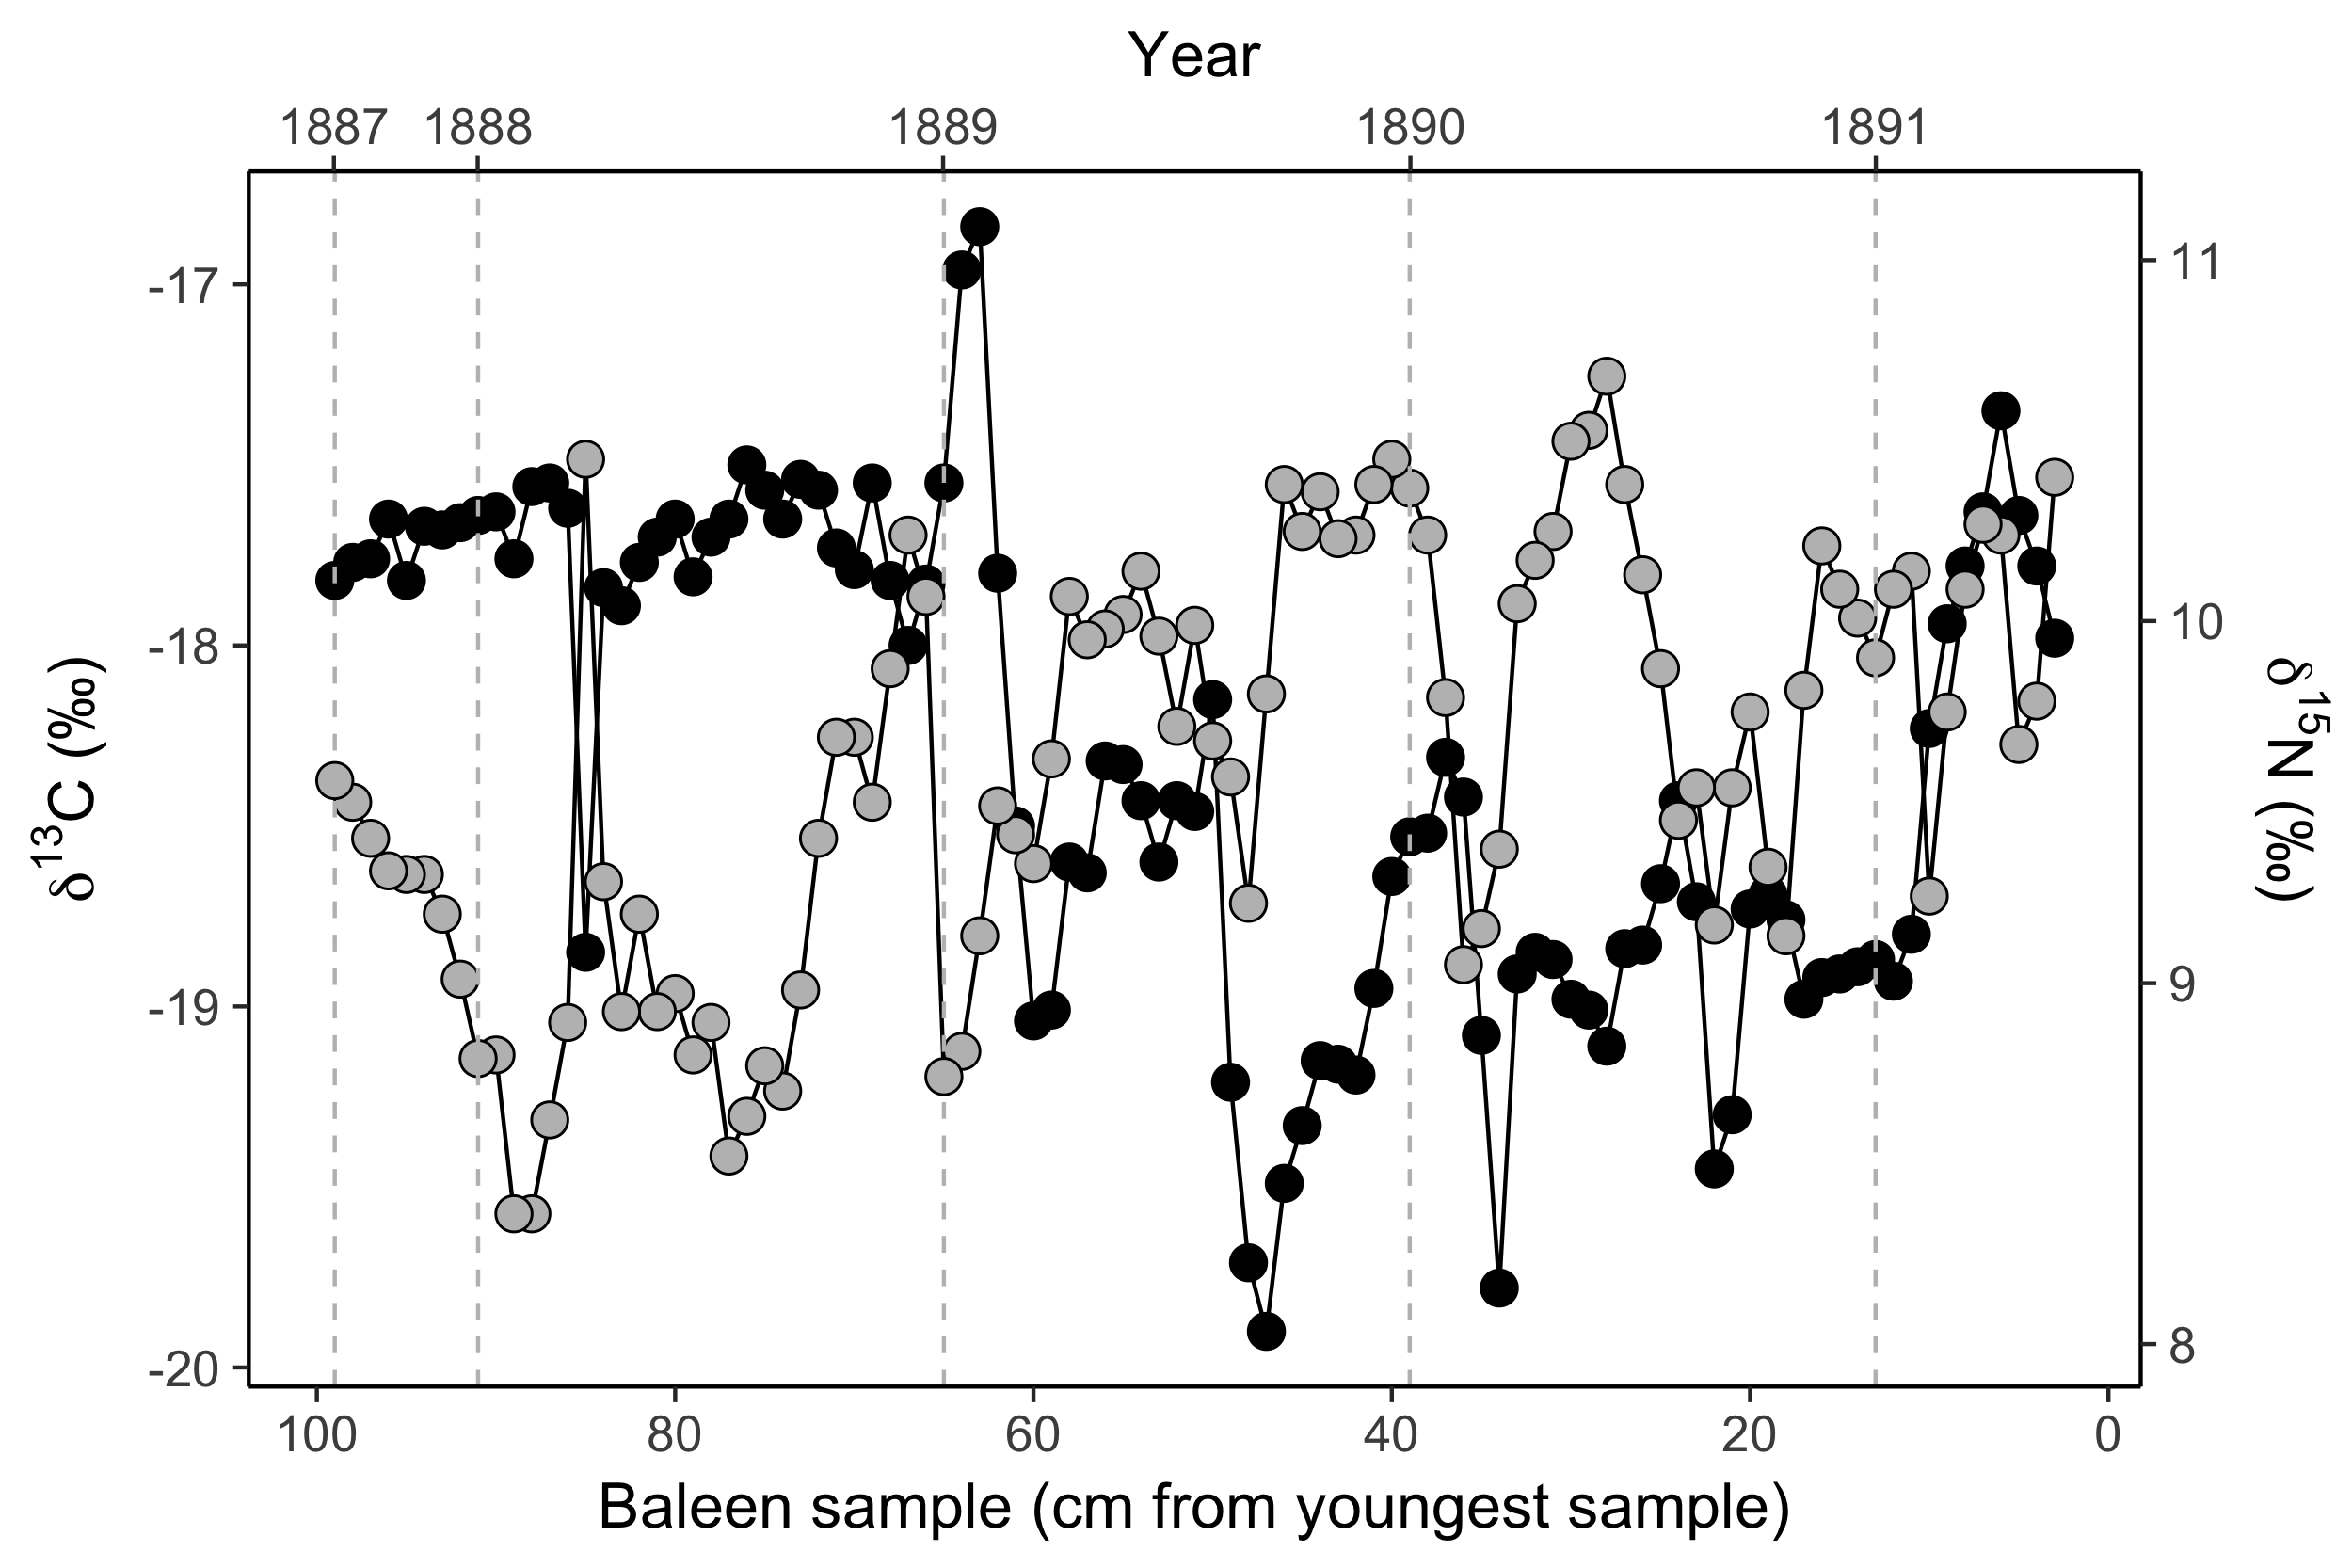
\includegraphics[width = \linewidth]{figures/Figure-1-raw-dC-dN-data.png}
  \caption{Variation in stable isotope values in the NHM blue whale, expressed as $\delta^{13}$C (black circles, left y-axis) and $\delta^{15}$N (grey circles, right y-axis). Samples were taken longitudinally through the baleen plate (n = XX samples from a single baleen plate for both isotopes) of the NHM blue whale exhibits strong annual periodicity and cross-correlation (Figs. S1 and S2) in both isotopes as well as a change in the mean and magnitude of the cycles during 1889 (approximately at sample 30cm). Approximate relationship to years assuming a growth rate of 13.5 cm y$^{-1}$ is shown on the upper x-axis, and year boundaries are indicated by vertical dotted grey lines.}
  \label{fig1}
\end{figure}

% Krill has a very similar isotopic composition to phytoplankton

Relating marine animal tissue isotopic compositions to likely locations is complicated by both a lack of spatial reference values, and because the isotopic composition of phytoplankton at the base of marine food webs varies in both space and time \cite{west2006stable}. %line 82 add ref mentioned by reviewer 1
We approach these problems using newly developed, temporally dynamic models of $\delta^{13}$C values in the global ocean\cite{magozzi2017using} (Fig. S3), coupled to an agent-based model of whale movements (see Supplementary Methods; Table S1; Fig. S5) to simulate time series of $\delta^{13}$C values expected under differing movement behaviours and in differing parts of the known geographic range of blue whales. 
We then compare simulated profiles (Figs. \ref{fig2}, \ref{fig3} and Fig. S4) with the measured isotopic profile of the blue whale's baleen (Fig. \ref{fig1}) to identify the most likely movement history.
We assume continued ingestion of new protein throughout the year. 
Other mysticete whales fast during migrations and during winter, relying on stored lipid reserves to meet metabolic demands, but blue whales are too large to stop feeding for long periods; \cite{busquets2017estimating,silva2013north}).
%Can we back this up? Are we more saying that we think they need protein to maintain tissue turnover but could meet energetic demands form stored lipids?

%SOME indirect evidence for grey whale continued feeding through migrations -


% figure 2
\begin{figure}
  \centering
  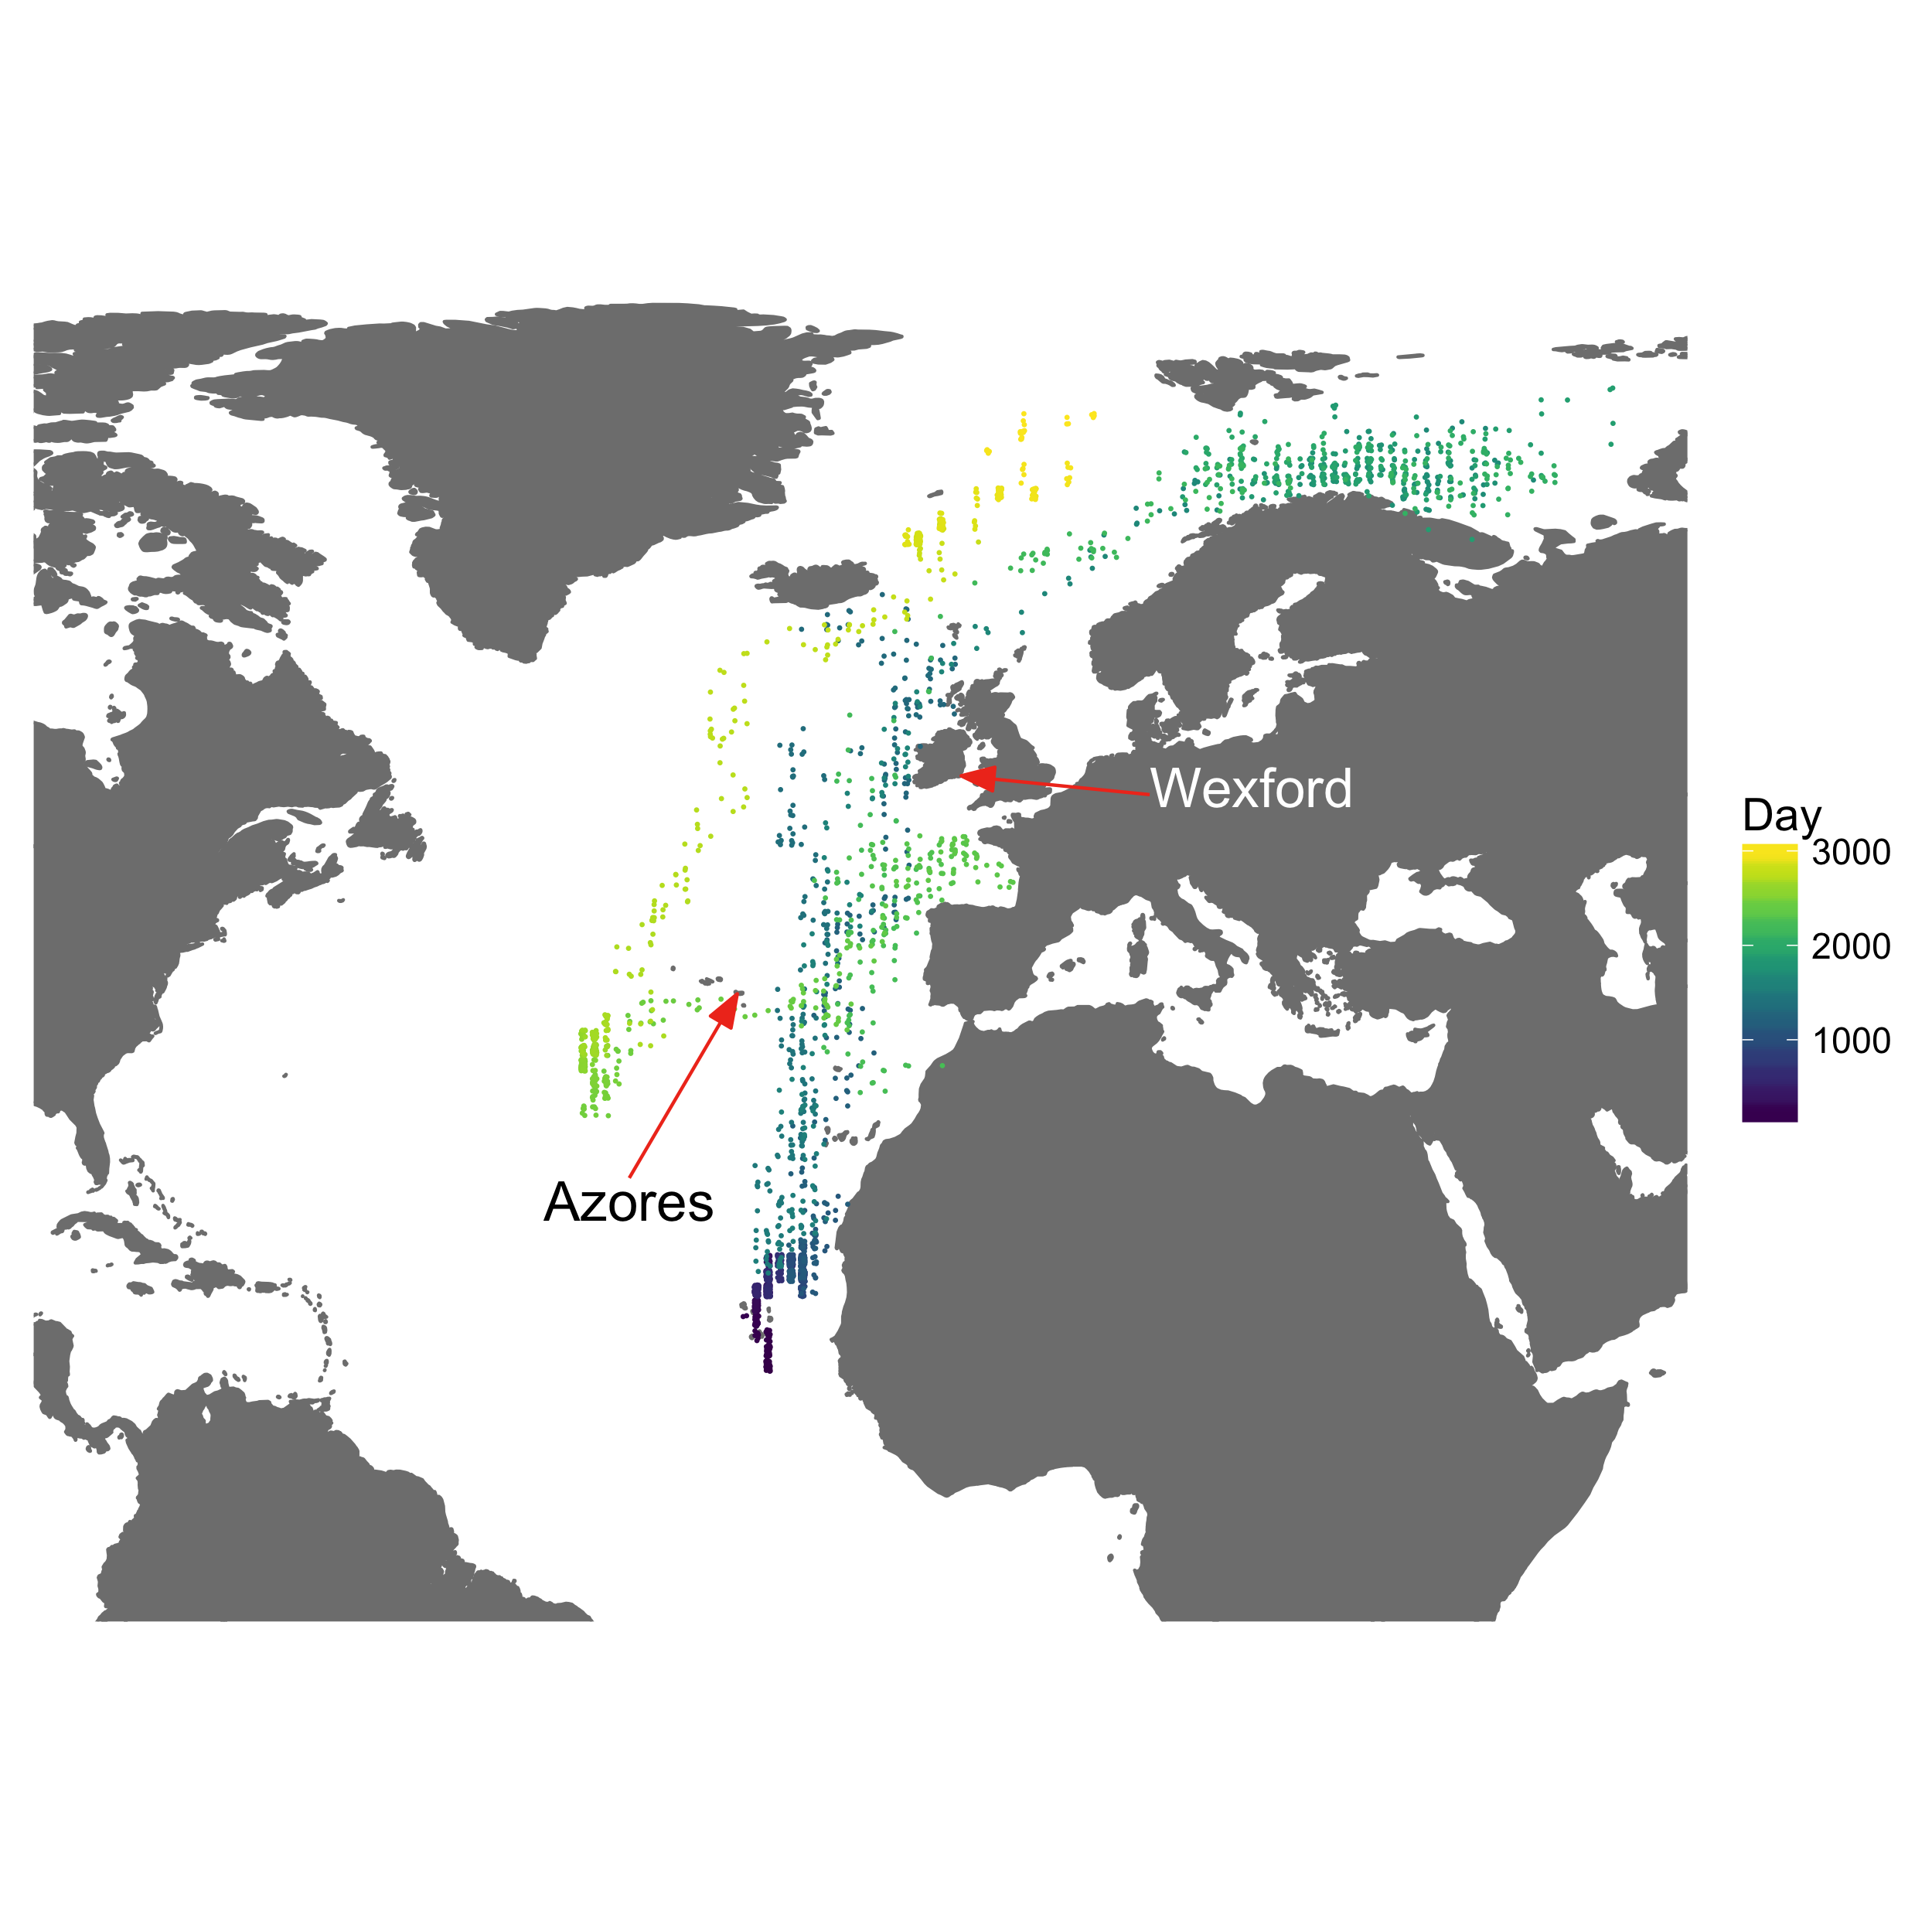
\includegraphics[width = \linewidth]{figures/Figure-2-migratory-model-full-map.png}
  \caption{Simulated tracks from the migratory movement model (2250 days for each of 50 replicates) with simulated day indicated by colour illustrating the residency period from Ireland to the Norwegian/Barents Sea followed by a migratory period and year spent near the Azores (as indicated by an arrow) and/or Canary Islands before returning north prior to stranding in Wexford, Ireland 1891 (as indicated by an arrow). }
  \label{fig2}
\end{figure}

% figure 3
\begin{figure}
  \centering
  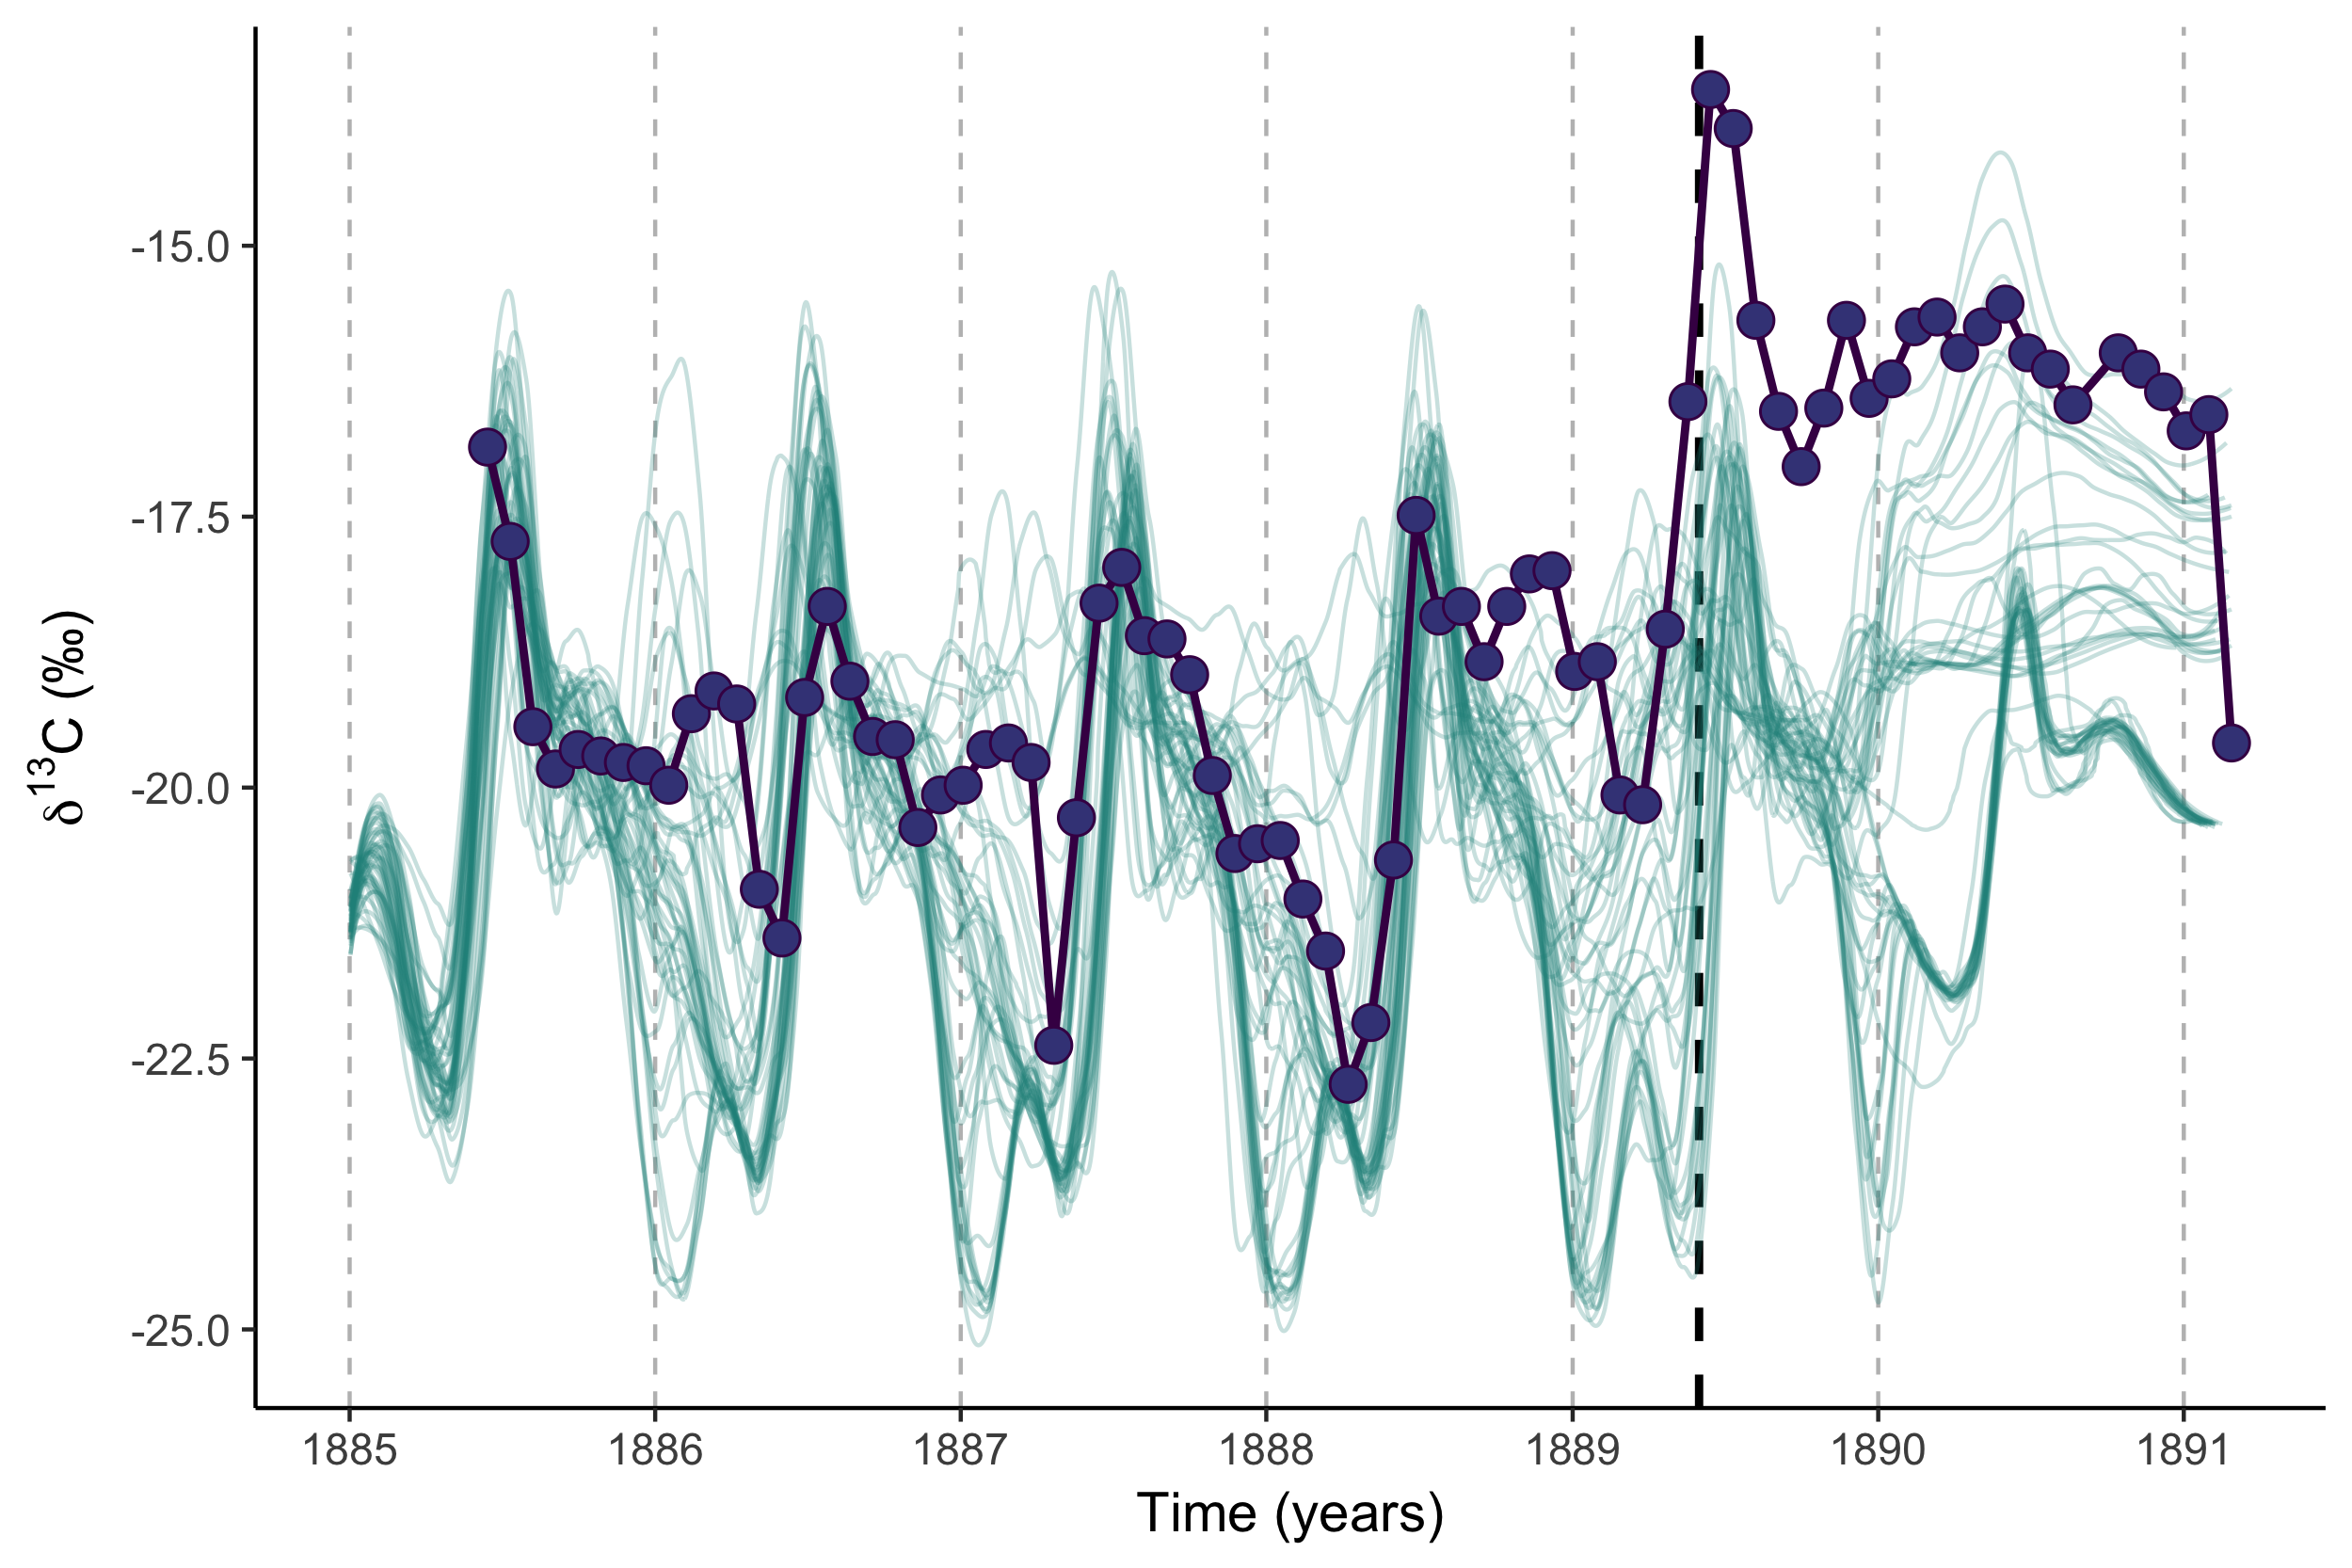
\includegraphics[width = \linewidth]{figures/Figure-3-migratory-model-d13C.png}
  \caption{Correlations among $\delta^{13}$C data from 50 movement simulations (green) and empirical data from baleen (blue). Across the 50 simulations, the correlation coefficient between z-score transformations of empirical and time-matched simulation values had a mean of 0.48 ($sd = 0.2$), 49 of them were positive, and 39 of the 50 Pearson correlation tests had a p-value less than the Bonferroni corrected value of 0.001 ($p = 0.05/50 = 0.001$). The initiation of the southward migration in the late spring of 1889 is indicated by the vertical broken line. The standard deviation of the empirical data have been rescaled by a factor of three so as to better visualise the correlation because, as a consumer, the whale is expected to integrate and attenuate the fluctuations in its diet, and the end points of the simulations and empirical data have been aligned to coincide.}
  \label{fig3}
\end{figure}
 
The relatively positive and seasonally-invariant $\delta^{13}$C values seen during behavioural phase one are only found in subtropical areas of the North Atlantic.  
Our simulations show high variance during this period (Fig. \ref{fig3}), reflecting a range of possible locations for the whale, although areas around the Cape Verde Islands, and potentially to the west of the Azores (Fig. \ref{fig2}), most closely match the measured profile. 
The whale remained in these warm waters for at least two full years. 
During behavioural phase two, starting at an approximate age of 5-6 years, the observed low $\delta^{13}$C values imply that the whale is foraging in colder, more northerly latitudes. 
The pronounced cyclical variations in $\delta^{13}$C values are characteristic of the isotopic expression of the spring phytoplankton bloom in northern waters \cite{magozzi2017using}.  

We simulated 1000 individual movement patterns and compared resulting simulated baleen $\delta^{13}$C records to the measured records with simple linear regressions. 
Simulated baleen $\delta^{13}$C profiles produce a good fit to measured profiles, the median $r^2$ value across 1000 simulated profiles was 0.49, and the maximum was 0.74 (Fig. S6, distribution of $r^2$ values). 
The top 10\% best fitting simulated profiles are shown in Fig. \ref{fig2} [line plot top 10\%). 
Best fitting models predict juvenile residency in the Cape Verde region in behavioural phase 1. 
Behavioural phase 2 is best simulated by seasonal migrations between summer foraging in northern areas in the Norwegian Sea/Barents Sea/Iceland region, and winter foraging in a broad region between the UK and sub-tropical waters. 
Best fitting models in general predicted a greater latitudinal foraging range, and foraging in more northerly waters (Supplementary materials Fig. S7 [boxplots and kernel density plots]).

%line 112 - 122 para
The last 500 days of the whale's life are difficult to simulate. 
Beginning in the winter of 1889/1890, the observed $\delta^{13}$C profile is relatively depleted, and remains constant for approximately six months, before increasing rapidly in the winter of 1890/1891. 
Depleted $\delta^{13}$C values are found in northern waters that show large temporal fluctuations in $\delta^{13}$Cplk values [fig SX residency plot], and the observed values cannot be simulated purely from movements within the known geographic range.
We infer that the $\delta^{13}$C record in the last period of life reflects the physiological demands of pregnancy, as similar increases in $\delta^{13}$C values have been seen in pregnant South American sea lions\cite{cardona2017temporal}. 
We suggest that the constant, depleted $\delta^{13}$C values reflect use of carbon reserves assimilated in northern latitudes during 6-8 months residency in low latitude waters. 
After six months the whale began feeding in low latitude waters producing a dramatic increase in $\delta^{13}$C values and began a final migration north. 
Blue whales have a 10-12 month gestation period, with calving occurring in sub-tropical waters, and calves are weaned after 6-7 months\cite{handbook}. 
The proposed timescale of pregnancy around early spring 1889, birth in spring 1890, residency in warm waters through the whole of 1890 with feeding resuming in the second half of 1890 and eventual stranding during the return to northern feeding grounds in early 1891, is therefore consistent with the known reproductive ecology of blue whales. 



%Possibly more interesting now to talk about juvenile behaviour and potential for prolonged residency in warm waters  - implications for interactions with tourist / shipping etc.

%Kernel density plot gives a visualization of proportional amount of time we infer the whale might have spent in each region
 
Conventional wisdom suggests that baleen whales migrate each year from feeding grounds near the poles in summer, to overwintering and breeding grounds nearer the equator\cite{corkeron1999baleen,lockyer1981migration}. 
However, a growing body of evidence suggests that not all whales migrate to subtropical waters each year, with some remaining at high latitudes year round\cite{mcdonald2006biogeographic}. %line 127
Our results support this conclusion. 
Interestingly, there is still a resident%line 128
 population of blue whales in the regions indicated by our model, and females still breed in the subtropical waters near the Azores\cite{reilly2008balaenoptera}. 
Whaling was an intense pressure for blue whales during the period we are analysing. 
Before whaling in the North Atlantic began in 1868\cite{reilly2008balaenoptera}, there were 10,000-15,000 blue whales in the region\cite{sigurjonsson1995life}. 
In the early 20th century, fisheries moved outside the area because stocks were so depleted\cite{reilly2008balaenoptera}; during this period over 12,000 blue whales were landed\cite{sigurjonsson1995life}. 
The NHM blue whale thus represents an individual from a species at the brink of extinction.
Our data suggest that the spatial ecology of blue whales in the North Atlantic has remained similar for more than 100 years, despite dramatic changes in anthropogenic pressures. % line 137 and 139

This is the first quantitative evidence of historical individual-level movement behaviours in blue whales. %line 140-141
Our novel simulation modeling removes a long-standing limitation in stable isotope ecology, and can be applied to stable isotope records from any incrementally-grown tissue to estimate most likely individual movement behaviours over multiple years. 
Such techniques can also be applied to extinct species behaviours and used to understand how populations were affected by past pressures such as hunting, and present-day pressures such as global change. 
Finally, our results highlight that museums represent a vast, mostly untapped, source of individual-level spatial ecology information. %line 147-149

\section{Methods}
%<3000 words
% no figures no tables

\subsection{Stable isotope extractions from baleen}
Baleen was collected from the Natural History Museum, London (specimen NHMUK.1892.3.1.1). 
The baleen plate was cleaned with ethanol to remove surface contaminants. 
{\raise.17ex\hbox{$\scriptstyle\sim$}}1mg samples of keratin powder were then collected from the plate using a hand-held drill and grinding bit. 
77 samples were taken at 1cm intervals, 0.5cm from the outer edge of the plate, starting at the proximal section which contains the most recent tissue. 
Baleen grows at a constant rate, so the samples are equally spaced through time\cite{best1996stable}. Carbon and nitrogen isotope analysis was performed simultaneously via continuous-flow isotope ratio mass spectrometry at the National Oceanographic Centre (Southampton, UK), using a Vario Isotope select elemental analyser, coupled with Isoprime 100 isotope mass spectrometer. 
Replicates using internal laboratory standards (L-glutamic acid (C), Glutamic acid (CT standard), acetanilide and protein standard OAS) were used for quality control and calibration. 
C:N ratios for samples ranged from 3.28\text{\textperthousand} to 3.72\text{\textperthousand}, well within the acceptable theoretical range for pure keratin ($3.4\pm0.5$) allowing for comparison among samples\cite{hobson1998stable}. 
 
\subsection{Time calibrating stable isotope profiles}
Seasonal migrations across isotopic gradients induce cyclical variations in the isotopic composition of baleen, the distance between cycles reflecting growth rates\cite{hobson1998stable,busquets2017estimating}. 
Clear periodicity was evident in $\delta^{15}$N values across the entire baleen plate, and in $\delta^{13}$C values in the most distal (oldest) 65cm of the plate. 
We calculated isotopic periodicity within the baleen sample using Fourier Transform analysis\cite{cardona2017temporal} (Fig. S1), revealing a consistent growth rate of 13.5$cmy^{-1}$ which is remarkably similar to the mean isotope-derived baleen growth rates of $15.5 \pm 2.2cmy^{-1}$ estimated for six recent blue whales from the Californian Pacific\cite{busquets2017estimating}.  
Therefore we dated the youngest baleen sample as 1st March 1891, 24 days prior to the stranding date, 25th March 1891. 
Cross-correlation analysis demonstrated a strong negative covariance between $\delta^{13}$C and $\delta^{15}$N values within behavioural phase one (oldest 60cm of the baleen plate), but no relationship between $\delta^{13}$C and $\delta^{15}$N values during behavioural phase two (Fig. S2).
 
\subsection{Baseline isotope comparisons}
Isotope-enabled biogeochemical ocean models\cite{magozzi2017using,schmittner2016complementary} were used to characterize the isotopic composition of phytoplankton expected in different potential foraging grounds (Fig. S3). 
Annual average $\delta^{15}$N POM (particulate organic matter) values were provided by Somes (pers.comm) based on a 5$^{\circ}$ resolution biogeochemical model (Fig. S3). 
$\delta^{13}$C POM values were simulated at 1$^{\circ}$ and monthly resolution using an isotopic extension to the NEMO-MEDUSA ocean biogeochemical model\cite{magozzi2017using,yool2013medusa}. 
Simulated  $\delta^{15}$N POM values are relatively positive in the northeast Atlantic north of c. 60$^{\circ}$N, and relatively negative in the central and southern North Atlantic. 
Annual average $\delta^{13}$C POM values largely vary with latitude, with more negative values in more northerly regions. 
In the central North Atlantic, $\delta^{13}$C POM values are relatively positive in the west, reflecting warm gulf stream waters (Fig. S3). 
The isotopic composition of carbon in phytoplankton also varies through seasons as isotopic fractionation of carbon during photosynthesis is strongly influenced by sea surface temperature\cite{magozzi2017using,laws1995dependence}.
Thus temporal variations in $\delta^{13}$C POM values were superimposed on latitudinal gradients. 
The scale and nature of temporal variation in $\delta^{13}$C POM values also varies with latitude, with higher latitude seas showing greater intra-annual variation in $\delta^{13}$C POM values linked to strongly seasonal phytoplankton growth dynamics. 
We therefore used monthly simulated $\delta^{13}$C POM values to simulate the isotopic expression of phytoplankton expected to be encountered by whales exhibiting differing movement behaviours.
 
\subsection{Agent-based whale movement model}
We simulated the movement of the whale with the likelihood, direction, and extent of movement influenced by behavioural state, sea surface temperature, water depth, and phytoplankton concentration (as a proxy for zooplankton food availability). 
At each time point and location in the simulations, we extracted phytoplankton $\delta^{13}$C values from the spatio-temporal model\cite{magozzi2017using} resulting in a range of simulated isotopic profiles for different migration patterns and foraging areas (Figs 2, 3, and S4). 
Movement was coded as a set of probabilistic rules. 
The parameters for these were taken from the literature on blue whale behaviour (e.g.\cite{handbook}). 
All terms were expressed as probability distributions allowing us to introduce individual variability. 
 
In the models, the likelihood of movement, direction (north, south, east, west, northeast, northwest, southeast, or southwest) and extent (1$^{\circ}$ or 2$^{\circ}$ in km) of movement are all influenced by the following. 
(i) Behavioural state (migrating north, migrating south, foraging, or nursing). 
Northerly migrations were possible only in spring, and southerly migrations in autumn. 
Foraging was possible at any time of year, and was triggered when whales encountered high concentrations of plankton. Nursing occurred at temperatures between 18 and 25$^{\circ}$C only. 
(ii) Sea surface temperature\cite{yool2013medusa} ($^{\circ}$C). 
When migrating north, whales were more likely to move towards lower temperatures provided they were above the minimum temperature threshold (3$^{\circ}$C); whereas whales migrating south sought warmer waters. 
(iii) Water depth (m; from the General Bathymetric Chart of the Oceans (GEBCO) global bathymetry dataset). 
Whales were less likely to move into waters less than 400m deep, and increasingly unlikely to move into even shallower waters. 
(iv) Phytoplankton concentration ($mmolNm^{-3}$, for combined diatom and non-diatom communities\cite{yool2013medusa}). 
This was included as a proxy for zooplankton food availability. 
Whales are more likely to move towards (or remain within) areas of high phytoplankton density, particularly during the foraging behavioural state. 
 
We simulated the isotopic expression expected for (a) residency in each known hotspot for blue whale sightings or historic hunting grounds in the North Atlantic (Norwegian/Barents Sea, West Ireland, Canaries/Azores and Mid Atlantic Ridge\cite{mcdonald2006biogeographic,reilly2008balaenoptera,sigurjonsson1995life} ; Fig S4); (b) seasonal migration between high sub-Arctic latitudes and temperate latitudes around the British Isles and (c) seasonal migration between high latitudes and subtropical latitudes. 
For a full description of the model and its parameters see Supplementary Methods: Fig. S5 and Table S1. 
We simulated whale movements 50 times for each scenario and 30 times for each residency hotspot (Fig. S4). 
For each movement simulation we extracted phytoplankton $\delta^{13}$C values at each time point and location from the models described above\cite{magozzi2017using}. 
We then compared the simulated stable isotope profiles (Fig. \ref{fig3}) to the profile of the blue whale (Fig. \ref{fig1}).
 
\subsection{Data Availability}
Data are available from Zenodo doi: [DOI will be added on acceptance]. 
R code is available from GitHub (github.com/ALJackson/blue-whale-bes).

% References

\bibliographystyle{nature}
\bibliography{blue-whale}

\section{Supplementary Information}
Supplementary Information is linked to the online version of the paper at www.nature.com/nature.

\section{Acknowledgments}
% adjectives not allowed!
This work was funded by the British Ecological Society (grant: 5771/6815). 
We thank C.J. Somes for providing  $\delta^{15}$N POM data.

\section{Author contributions}
% rough draft at present feel free to edit
CT, NC, AJ, RS, and KC collected baleen from the NHM collections. 
KC and CT extracted and analysed samples.
CT created the movement model.
EC, NC and RS helped parameterise the model.
AJ created the figures. 
CT, NC and EC wrote the paper.
All authors edited drafts and approved the final version.

\section{Author information}
Reprints and permissions information is available at www.nature.com/reprints.
The authors declare no competing financial interests.
Correspondence and requests for materials should be addressed to natalie.cooper@nhm.ac.uk.

%\section{Figure legends}

%\section{Figures}

\end{document}